%======================================================================
\NEWSEC
%======================================================================

\subsection{\ssRecentParticles}

%----------------------------------------------------------------------
\begin{frame}[fragile,label=ss-recent-particles] 
  \secframetitle{\ssRecentParticles}
  \framesubtitle{Cello supports Particles!}

\begin{minipage}{2.5in}
\begin{itemize}
\item user-defined types
\begin{itemize}
        \item  declared in input parameter file
        \item  \bluecode{"trace"}: tracer particles
        \item  \bluecode{"dark"}: dark matter particles
        \item  others defined as needed
\end{itemize}
\item each with own list of attributes
\begin{itemize}
        \item  position (\bluecode{"x"},\bluecode{"y"},\bluecode{"z"})
        \item  velocity (\bluecode{"vx"},\bluecode{"vy"},\bluecode{"vz"})
        \item  mass (\bluecode{"mass"})
        \item  id (\bluecode{"id"})
        \item \textit{integer} (8-,16-,32-,64-bit)
        \item \textit{float}   (32-, 64-, 128-bit)
        \end{itemize}
\item constant attributes available
\end{itemize}
\end{minipage} \
\begin{minipage}{2.0in}
%\ANIMATEGRAPHICS{width=1.25in}{20}{Images/Trace/Trace-0}{000}{010}
\end{minipage}
\end{frame}

%======================================================================

\begin{frame}[fragile,label=ss-recent-particles] 
  \secframetitle{\ssRecentParticles}
\framesubtitle{How \code{Particle} objects store particle data}
\begin{minipage}{1.8in}
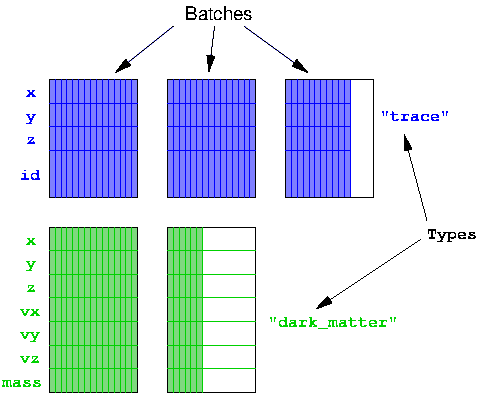
\includegraphics[width=2.0in]{particles-design.pdf} \ \\
\end{minipage} \ 
\begin{minipage}{2.5in}
\begin{itemize}
\item multiple particle \textit{types}
\item particles allocated in \textit{batches}
\begin{itemize}
\item fixed size arrays
\item fewer new/delete operations
\item efficient insert/delete operations
\item potentially useful for GPU's
\end{itemize}
\item batches store particle \textit{attributes}
\begin{itemize}
\item (position, velocity, mass, etc.)
\item 8,16,32,64-bit integers
\item 32,64,128-bit floats
\end{itemize}
\end{itemize}
\end{minipage}
\begin{itemize}
\item particle positions may be floating-point or integers
\begin{itemize}
\item floating-point for storing global positions
\item integers for \code{Block}-local coordinates
\begin{itemize}
\item solves reduced precision issue for deep hierarchies
\item less memory required for given accuracy
\end{itemize}
\end{itemize}
\end{itemize}
\end{frame}

%----------------------------------------------------------------------
%
% Review of Particles in Cello
%
%   Particles that move between blocks are handled by Cello
%
%   Cello handles moving particles
%     4^3 array
%     one-pass through particles to sort and scatter
%     particles
%

\begin{frame}[fragile,label=ss-recent-particles] 
  \secframetitle{\ssRecentParticles}
  \framesubtitle{Particle communication between Blocks}
\begin{itemize}
\item communication is required when particles move outside a Block 
\item this is done using a 4x4x4 array
\begin{itemize}
\item array contains pointers to ParticleData (PD) objects
\item one PD object per neighbor Block
\end{itemize}

\end{itemize}
\begin{minipage}{1.8in}
%\includegraphics<1>[width=2.0in]{particle-refresh-0.pdf}
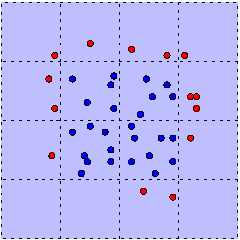
\includegraphics[width=2.0in]{particle-refresh-2.pdf}
%\includegraphics<4>[width=2.0in]{particle-refresh-3.pdf}
%\includegraphics[width=2.0in]{particle-refresh-4.pdf}
\end{minipage} \ 
\begin{minipage}{2.7in}
\begin{itemize}
\item migrating particles are
\begin{itemize}
\item \code{scatter()}-ed to PD array objects
\item sent to associated neighbors
\item \code{gather()}-ed by neighbors
\end{itemize}
\item one sweep through particles
\item one communication step per neighbor
%\item similar for refinement / coarsening
\end{itemize}
\end{minipage}
\end{frame}

%----------------------------------------------------------------------
%  
%   Class structure of particles in Cello mirrors Field classes
%
%   Particle: particles as seen by application
%     ParticleDescr: ``descriptor'' class defining particle parameters
%     ParticleData: ``data'' class containing block particle data
%

%\begin{frame}[fragile,label=ss-recent-particles] 
%  \secframetitle{\ssRecentParticles}
%  \framesubtitle{Class structure of particles}
%
%\end{frame}

%----------------------------------------------------------------------

\begin{frame}[fragile,label=ss-recent-particles] 
  \secframetitle{\ssRecentParticles}
  \framesubtitle{Particle type parameters}
Particles are declared in the input parameter file using the Particle group

\begin{tabbing}
\code{xxxxxx}\=\code{xxxxx}\=\code{xxxxxxxxxxxxxx}\=\kill
\code{Particle \{} \\
\>    \code{list = ["trace"];} \\
\\
\>    \code{trace \{} \\
\> \>     \code{attributes = ["id", "int64",} \\
\> \> \> \code{\ "x", "single",} \\
\> \> \> \code{\ "y", "single",} \\
\> \> \> \code{\ "z", "single"];} \\
\> \>      \code{position = ["x","y","z"];} \\
\> \>      \code{batch\_size = 2000; } \\
\>    \code{\} } \\
\code{\} }
\end{tabbing}
\end{frame}

%----------------------------------------------------------------------

\begin{frame}[fragile,label=ss-recent-particles] 
  \secframetitle{\ssRecentParticles}
  \framesubtitle{Particle type parameters}
  \small
\begin{tabbing}
\code{xx}\=\code{xx}\=\code{xxx}\=\kill
\code{Particle \{} \\
\>    \code{list += ["dark"];} \\
\\
\>    \code{dark \{ } \\
\> \> 	  \code{attributes = } \\
\> \> \> \code{  [ "x", "double",  "y", "double", "z", "double",} \\
\> \> \> \code{   "vx", "single", "vy", "single","vz", "single",} \\
\> \> \> \code{   "ax", "single", "ay", "single","az", "single"];} \\
\> \>     \code{constants = ["mass", "single"];} \\
\> \>     \code{position = [ "x", "y", "z"];} \\
\> \>     \code{velocity = ["vx","vy","vz"];} \\
\> \>     \code{groups = ["has\_mass"];} \\
\>      \code{\} } \\ 
\code{\} }
\end{tabbing}
\end{frame}
%----------------------------------------------------------------------
%  Runs were made with tracer particles to ensure parallel scaling
%
%
%   - [ ]  include 1705-BW slides
%

\begin{frame}[fragile,label=ss-recent-particles] 
  \secframetitle{\ssRecentParticles}
  \framesubtitle{Parallel scaling test problem}
  \textbf{We tested basic \enzop\ hydrodynamics and particles scalability}
  \begin{minipage}{1.5in}
  \vspace{0.2in}
    \includegraphics<1>[width=1.5in]{de-2-3.png} \\
\ \\
    \includegraphics<1>[width=1.5in]{age-2-16.png}
  \end{minipage} \
  \begin{minipage}{2.75in}
    \vspace{0.1in}
    \begin{itemize}
    \item variation of ``array of Sedov Blast'' test
    \item letters instead of spheres
      \begin{itemize}
      \item inhibits lockstep coarsen/refine
      \end{itemize}
    \item one letter per Blue Waters core
    \item tested with/without tracer particles
    \item $32^3$ or $24^3$ cells per block
    \item among largest AMR runs ever done
      \begin{itemize}
      \item $256K$ fp-cores
      \item $1.7T$ cells; $0.7T$ (cells + particles)
        \item $50M$ Blocks
      \end{itemize}
      \item \enzo\ would require $ \ge 72GB$ / process
    \end{itemize}
    \end{minipage}
  
\end{frame}

\begin{frame}[fragile,label=ss-recent-particles] 
  \secframetitle{\ssRecentParticles}
  \framesubtitle{Particle weak scaling results}
%--------------------------------------------------  
\begin{center}
  \vspace{-0.1in}
  \begin{minipage}{4.50in}
    \begin{center}
%      \begin{minipage}{2in}
%    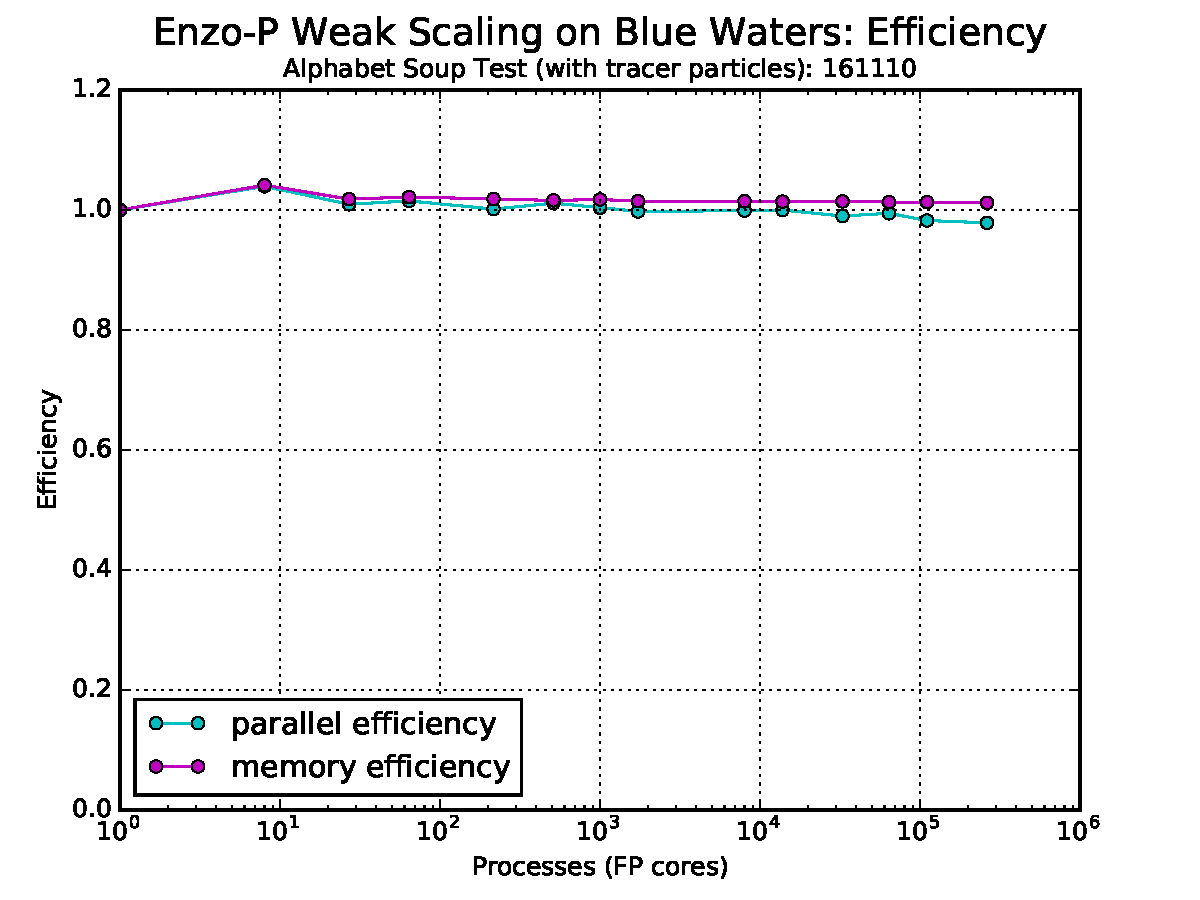
\includegraphics[width=2.0in]{scaling-efficiency-161110.pdf}
%    \end{minipage} \ 
      \begin{minipage}{4in}
    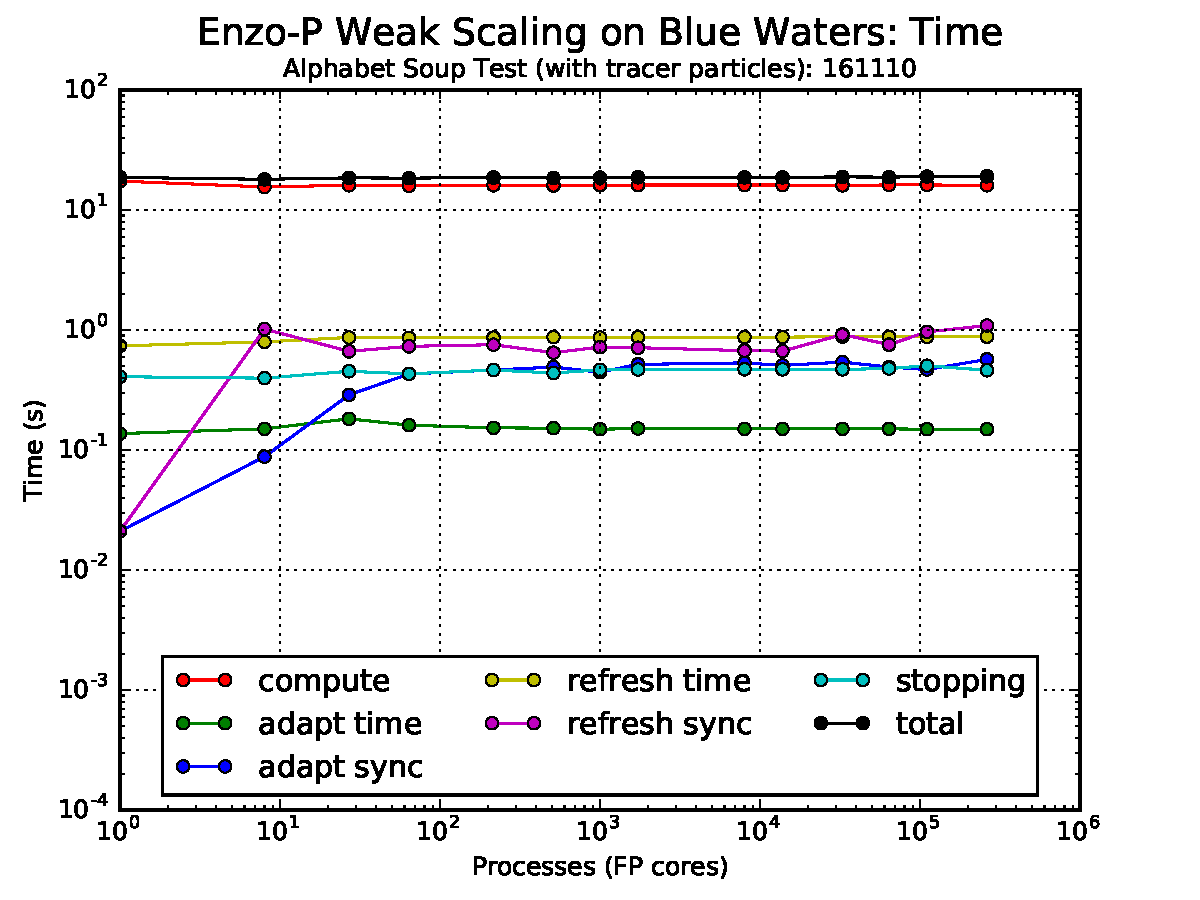
\includegraphics[width=4.0in]{scaling-time-161110.pdf}
    \end{minipage} \\
    \end{center}
  \end{minipage} \\
\end{center}
  
\end{frame}


